\chapter{座標轉換}
\subsection{導入虛擬場景}
將CAD檔轉入虛擬環境時,可能會以不理想的座標系及大小進入到環境為了解決這個問題,藉由找出空間中的體積及及慣性矩還有軸心,利用pySTLl將Cad檔座標矯正。\\
\begin{itemize}
%=----------Sigmoid      Function----------=%
\item 網格及法線的形成(圖.\ref{三角網格法線方向}):\\
STL文件表示的表面是封閉並連接的三角形網格,其中每條邊都是兩個三角形的一部分,並且不相交。對於一個三角形,可以通過頂點的順序和右手定則來決定,如果公共邊有不同的方向,就可以證明兩個三角形的法線是一致的。\\
\begin{figure}[hbt!]
\begin{center}
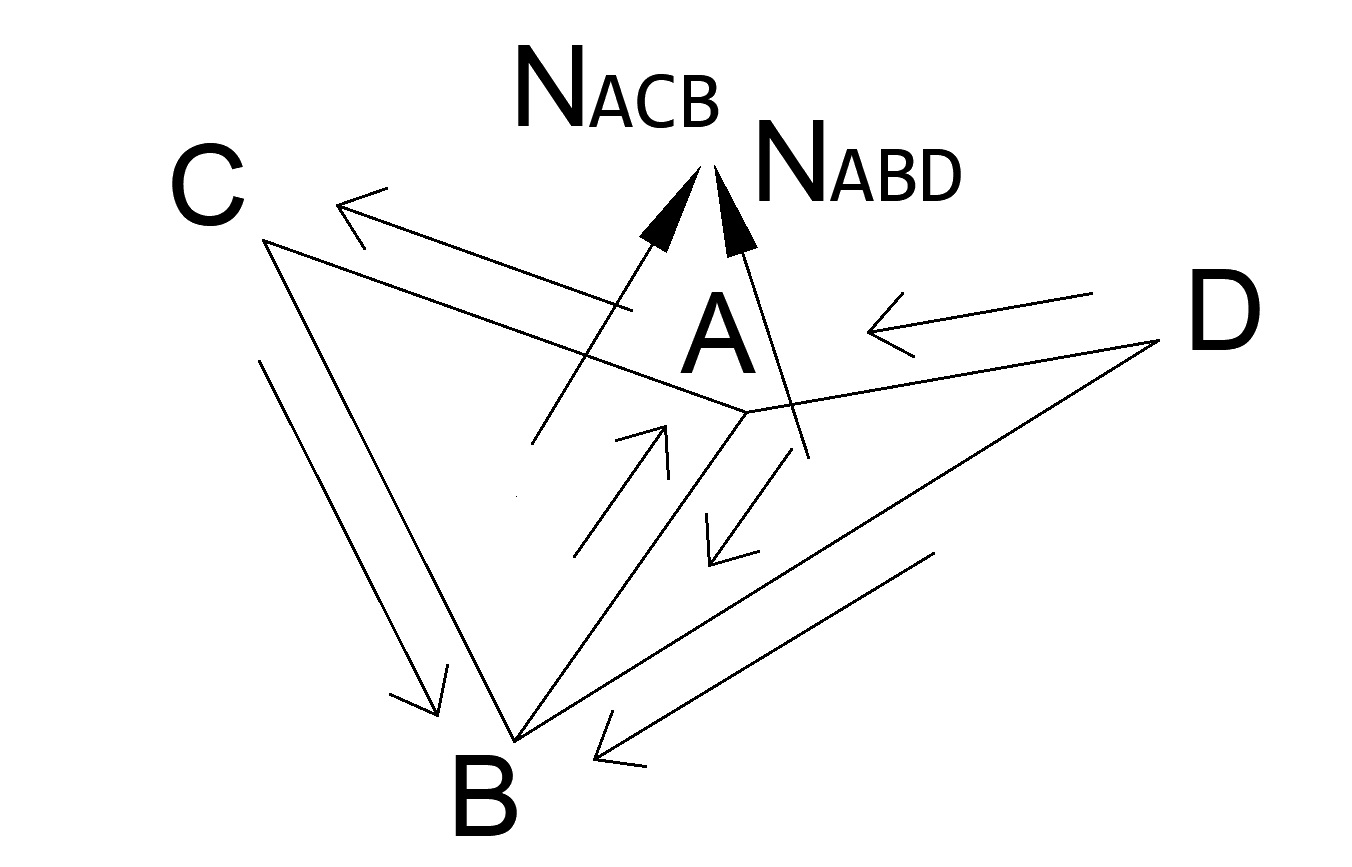
\includegraphics[width=16cm]{三角網格法線方向}
\caption{\Large 三角網格法線方向}\label{三角網格法線方向}
\end{center}
\end{figure}
\\
%=----------Softmax Function----------=%
\item 四面體體積(圖.\ref{3D體積的計算}):\\
在3D情況下,計算的基本單元為四面體,將原點與三角形的各個頂點連接形成一個四面體。三角形ACB具有法線NACB,由於原點 O 位於 NACB 的對面,因此這個四面體的值是正的,體積也可以由內積 OA $\cdot$ NACB 判斷。四面體體積為:\\
$$ V'_t = \frac{1}{6}(-x_3i y_2i z_1i + x_2i y_3i z_1i + x_3i y_1i z_2i - x_1i y_3i z_2i - x_2i y_1i z_3i + x_1i y_2i z_3i) $$
$$ V'_total= \sum_{i}V'_i$$

\begin{figure}[hbt!]
\begin{center}
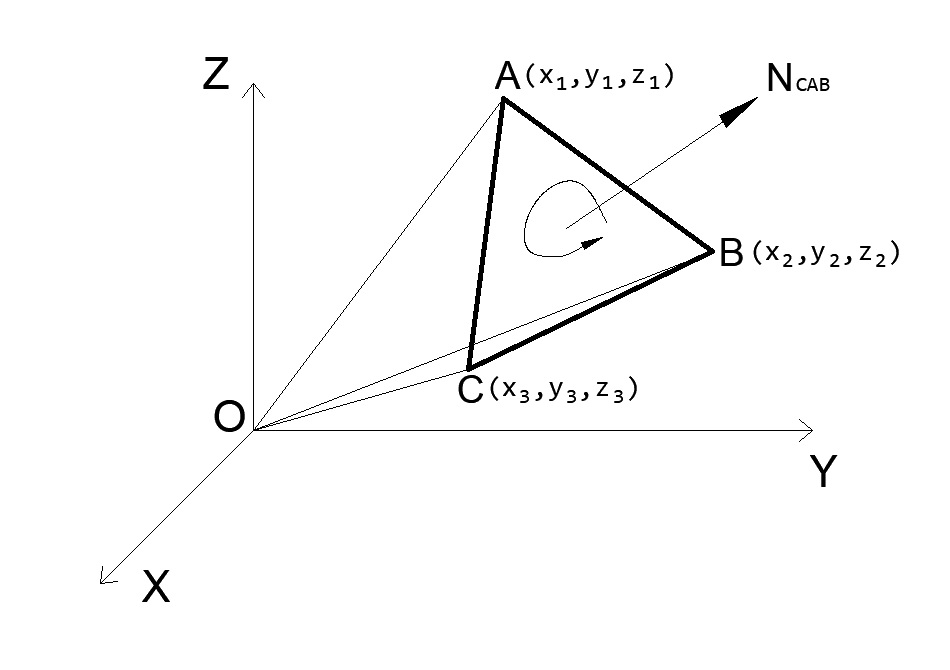
\includegraphics[width=16cm]{3D體積的計算}
\caption{\Large 3D體積的計算}\label{3D體積的計算}
\end{center}
\end{figure}
%=----------Relu Function----------=%
\item 空間裡的體積:\\
計算的特徵可以寫為帶有作標總和的基礎特徵形狀,並且可以以顯式倒出基本形狀,雖然這是一個很大的約束,但是在內部空間上具有積分形式都可以使用。\\
 p, q, r 為矩的階,中心矩可以從下列求解:\\

$$M_{pqr} = \iiint x^{p} y^{q} z^{r} \rho (x,y,z) \,dx\,dy\,dz$$
其中 $\rho (x,y,z)$ 是基礎形狀i的指示函數:\\
\begin{equation}
\label{eq6}
\rho (x,y,z) = \left\{
\begin{aligned}
1 & , & if (x,y,z) is inside the mesh\\
0 & , &              otherwise
\end{aligned}
\right.
\end{equation}
$S_i$ 是形狀i做有標記座標的體積的符號函數,積分可以重寫為每個基本形狀的積分之和:\\
$$M_pqr = \sum_{i} S_i \iiint x^{p} y^{q} z^{r} \rho_i (x,y,z) \,dx\,dy\,dz$$

由於物體內部的空間可以使用傅里葉變換,也能通過將積分分解為每個基本形狀的積分來計算。二維的傅里葉轉換或 3D 網格模型由傅里葉變換定義其指示函數:\\

$$ \Theta (u,v,w) = \iiint e^{-i (xu+yv+zw)} \rho (x,y,z) \,dx\,dy\,dz $$

\item 產生矩陣:\\
主軸是通過計算矩陣 S 的特徵向量獲得的,也稱為主成分分析 (PCA)。 將最大特徵值對應的特徵向量作為第一主軸。 第二個特徵值對應的下一個特徵向量是第二個主軸,以此類推。我們進一步確保三階矩 M300 和 M030 變換後是正的,為了使最終結果是唯一的。\\

我們通過 3D 模型的二階矩構造一個 3x3 矩陣:

\[ 
S=\begin{bmatrix} 
M_{200} & M_{110} & M_{101} \\
M_{110} & M_{020} & M_{011} \\
M_{101} & M_{011} & M_{022} 
\end{bmatrix}
\]

\item 總結:\\
pySTL中需要用到的體積和慣性矩去轉換質心,使用質點繞了座標軸即可調整物體的角度、移動與比例縮放,在上述的式子中可以得到出需要的解;\\

體積:$M_{000} = \frac{1}{6}(-x_3 y_2 z_1 + x_2 y_3 z_1 + x_3 y_1 z_2 - x_1 y_3 z_2 - x_2 y_1 z_3 + x_1 y_2 z_3) $\\

對x的一次矩:$M_{100} = \frac{1}{4}(x_1 + x_2 + x_3) M_{000} $\\

對x的一次矩:$M_{010} = \frac{1}{10}(x_1^{2} + x_2^{2} + x_3^{2} + x_1 x_2 + x_2 x_3 + x_1 x_3 ) M_{000} $\\

質點x軸位置:\\

$$M_{100} = (\frac{1}{4}(x_1 + x_2 + x_3)) M_{000}$$

質點y軸位置:\\

$$M_{010} = (\frac{1}{4}(y_1 + y_2 + y_3)) M_{000}$$

質點x軸位置:\\

$$M_{001} = (\frac{1}{4}(z_1 + z_2 + z_3)) M_{000}$$


\end{itemize}